\documentclass{article}
\usepackage[margin=1in]{geometry}
\usepackage[dvipsnames]{xcolor}
\definecolor{violet}{rgb}{0.56,0,1}
\definecolor{orange}{rgb}{1,0.5,0}
\definecolor{brown}{rgb}{0.65,0.16,0.16}
\definecolor{gray}{gray}{0.5}
\usepackage{tikz}

\usetikzlibrary{arrows.meta,decorations.markings}
\usepackage{multicol}
\usepackage{lmodern}
\usepackage{setspace}
\usepackage{amsmath}
\usepackage[T1]{fontenc}
\usepackage[utf8]{inputenc}
\usepackage{hyperref}  % For \url
\usepackage{url}       % For \url (not strictly needed if using hyperref)

\pagestyle{empty}




\begin{document}

    \begin{center}
    {\Huge\bfseries Vortex Æther Model (VAM)}\\[3pt]
    {\large\bfseries Unified Roadmap of Quantum, Gravity, and Topology}
    \end{center}
    \vspace{0.4cm}

    \noindent
    \textbf{Abstract:}
    \begin{spacing}{1.08}
        \noindent
        The Vortex Æther Model (VAM) unifies gravity, quantum mechanics, and particle physics as emergent phenomena of a knotted superfluid æther. Mass, time, charge, and all physical constants ($G$, $\hbar$, $\alpha$) are derived from vortex topology, swirl-induced pressure, and fluid geometry—without arbitrary postulates. This roadmap summarizes the logical flow and core results of the VAM paper series.
    \end{spacing}
    \vspace{0.4cm}

    \begin{center}


            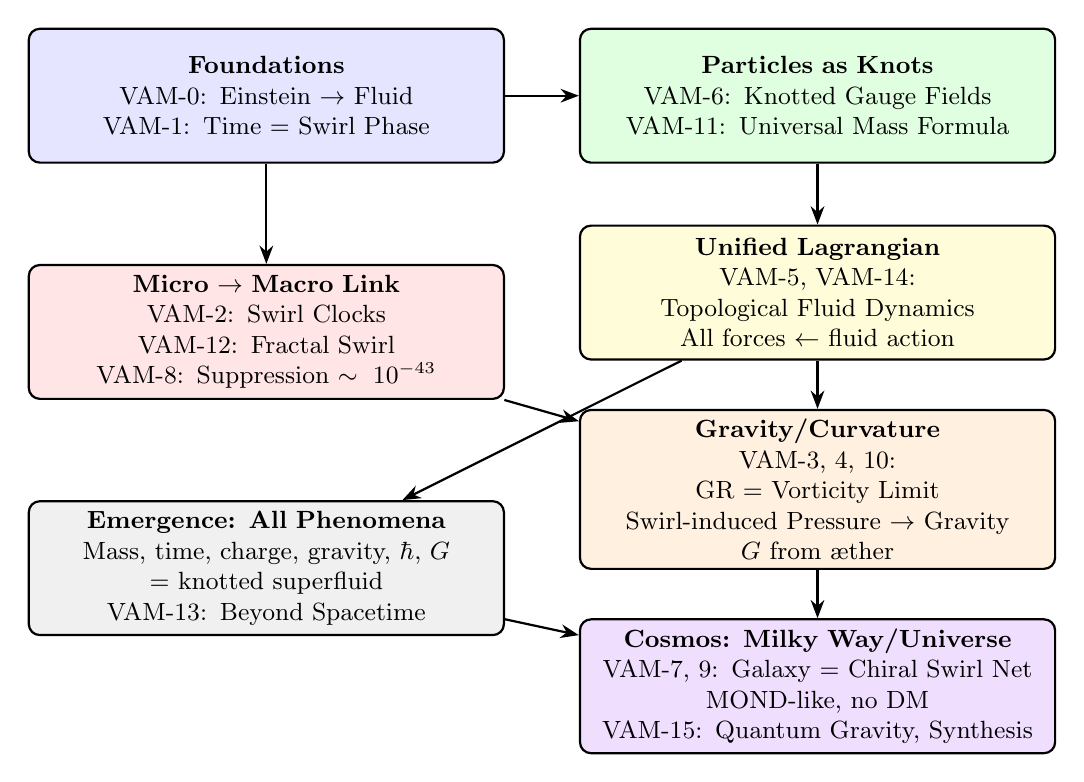
\begin{tikzpicture}[
                every node/.style={align=center, font=\small, text width=5.8cm, minimum height=1.7cm},
                node distance=2.4cm and 1.6cm,
                >=Stealth, thick
            ]

            {\Large\bfseries Vortex Æther Model (VAM): One-Page Research Roadmap}
% FOUNDATION
                \node[draw, rounded corners, fill=blue!10] (found) at (0, 0) {%
                    \textbf{Foundations}\\
                    VAM-0: Einstein $\to$ Fluid\\
                    VAM-1: Time = Swirl Phase
                };

% PARTICLE PHYSICS MODULE
                \node[draw, rounded corners, fill=green!12] (particle) at (7, 0) {%
                    \textbf{Particles as Knots}\\
                    VAM-6: Knotted Gauge Fields\\
                    VAM-11: Universal Mass Formula
                };

% LAGRANGIAN
                \node[draw, rounded corners, fill=yellow!15] (lagrangian) at (7, -2.5) {%
                    \textbf{Unified Lagrangian}\\
                    VAM-5, VAM-14:\\
                    Topological Fluid Dynamics\\
                    All forces $\leftarrow$ fluid action
                };

% MICRO-MACRO LINK
                \node[draw, rounded corners, fill=red!10] (micro) at (0, -3) {%
                    \textbf{Micro $\to$ Macro Link}\\
                    VAM-2: Swirl Clocks\\
                    VAM-12: Fractal Swirl\\
                    VAM-8: Suppression $\sim 10^{-43}$
                };

% GRAVITY
                \node[draw, rounded corners, fill=orange!12] (gravity) at (7, -5) {%
                    \textbf{Gravity/Curvature}\\
                    VAM-3, 4, 10:\\
                    GR = Vorticity Limit\\
                    Swirl-induced Pressure $\rightarrow$ Gravity\\
                    $G$ from æther
                };

% COSMOLOGY
                \node[draw, rounded corners, fill=violet!13] (cosmo) at (7, -7.5) {%
                    \textbf{Cosmos: Milky Way/Universe}\\
                    VAM-7, 9: Galaxy = Chiral Swirl Net\\
                    MOND-like, no DM\\
                    VAM-15: Quantum Gravity, Synthesis
                };

% EMERGENCE/ALL
                \node[draw, rounded corners, fill=gray!12] (emerg) at (0, -6) {%
                    \textbf{Emergence: All Phenomena}\\
                    Mass, time, charge, gravity, $\hbar$, $G$\\
                    = knotted superfluid\\
                    VAM-13: Beyond Spacetime
                };

% Connections
                \draw[->] (found) -- (micro);
                \draw[->] (found) -- (particle);
                \draw[->] (particle) -- (lagrangian);
                \draw[->] (lagrangian) -- (gravity);
                \draw[->] (lagrangian) -- (emerg);
                \draw[->] (micro) -- (gravity);
                \draw[->] (gravity) -- (cosmo);
                \draw[->] (emerg) -- (cosmo);

    \end{tikzpicture}

    \vspace{0.7cm}
    \noindent
    \textbf{Legend:} Each colored module is a VAM theme; major papers are bolded. Arrows show logical flow from foundations to universal predictions.

    \begin{multicols}{2}
        \footnotesize
        \textbf{Highlights:}
        \begin{itemize}
            \item \textbf{Gravity} is swirl-induced pressure, not spacetime curvature
            \item \textbf{Mass, charge, time, spin}: All emerge from vortex knot topology in the superfluid æther
            \item \textbf{Suppression factor} ($\sim 10^{-43}$): Explains why gravity is so weak compared to other forces (micro-to-macro vorticity coherence)
            \item \textbf{All fundamental constants derived:}
            \begin{itemize}
                \item \textbf{Newton's constant:} $G = \dfrac{C_e c^3 t_p^2}{r_c m_e}$
                \item \textbf{Planck's constant:} $\hbar = \rho_{\text{\ae}}^{(\text{mass})} r_c^5 C_e$
                \item \textbf{Fine structure:} $\alpha = \dfrac{2 C_e}{c}$
                \item \textbf{Æther density:} $\rho_{\text{\ae}} = \dfrac{2 m_e c^2}{3} \left(\dfrac{\alpha m_e c^2}{\hbar}\right)^2 r_e^3$
            \end{itemize}
            \item \textbf{Universal mass formula:} $m = \dfrac{\rho_{\text{\ae}}^{(\text{mass})} C_e^2 r_c^3}{c^2} \, \Xi(\ell, H, K)$
            \item \textbf{Unified action/Lagrangian:} All known forces as topological-fluid terms; gauge invariance and symmetry breaking have fluid analogs
            \item \textbf{Emergent quantum mechanics:} $\hbar$ and quantum phenomena from vortex energetics
            \item \textbf{Galaxy rotation (no dark matter):} Flat curves and MOND scaling from quantum microphysics
            \item \textbf{Time dilation and relativity:} Fluid-dynamical phase effects, not spacetime geometry
            \item \textbf{Testable predictions:} Rotational drag, vortex-core structure, critical speeds in superfluid analogs, gravitational lensing
            \item \textbf{Mathematical toolkit:} Fractal geometry, knot invariants, phase synchronization, coarse-graining
            \item \textbf{No arbitrary fits:} All parameters are geometric/topological, not empirical
        \end{itemize}
    \end{multicols}
    \end{center}


    \newpage


    \begin{tikzpicture}[scale=1.3, x=1cm, y=1cm]

        \def\a{0.8}
        \def\b{0.48}
        \def\N{7}
        \pgfmathsetmacro\maxangle{int(360*\N)}
        \foreach \t in {0,5,...,\maxangle} {
            \pgfmathsetmacro\radius{\a + \b * (\t/360)}
            \draw[very thick, blue!40!black]
            ({\radius*cos(\t)}, {\radius*sin(\t)}) --
            ({(\a+\b*(5/360)+\b*(\t/360))*cos(\t+5)}, {(\a+\b*(5/360)+\b*(\t/360))*sin(\t+5)});
        }


        \foreach \n/\name/\col in {
            0/{Planck core}/red,
            1.618/{electron}/blue,
            2.5/{up quark}/green!80!black,
            3.14/{neutrino}/gray,
            4.618/{proton}/orange,
            5/{neutron}/orange,
            6.8/{deuteron}/brown,
            7.6/{$g\sim10^{-43}$}/black,
            8.3/{galaxy}/violet
        }{
            \pgfmathsetmacro\theta{360*\n}
            \pgfmathsetmacro\radius{\a + \b*\n}
            \filldraw[fill=\col, draw=black]
            ({\radius*cos(\theta)}, {\radius*sin(\theta)}) circle [radius=0.14];
            \node[
                fill=white,
                draw=black,
                rounded corners,
                inner sep=1.2pt,
                font=\scriptsize,
                anchor=south
            ] at ({\radius*cos(\theta)}, {\radius*sin(\theta)+0.22}) {\name};
        }



        % EXPLICIT LEGEND ENTRIES (example)

        \node[anchor=west, gray] at (-6,1.5) {Suppression \& Gravity};
        \node[anchor=west, orange] at (-6,1) {Baryons \& Nuclei};
        \node[anchor=west, green!60!black] at (-6,-1) {Quarks \& Leptons};
        \node[anchor=west, red] at (-6,-1.5) {Core: $r_c, C_e, \rho_{\text{\ae}^{\text{(fluid)}}}$};
        \node[anchor=west, red] at (-6,-2) {\rho_{\text{\ae}^{\text{(mass)}}}$};
        \node[anchor=west, red] at (-6,-2.5) {\rho_{\text{\ae}^{\text{(energy)}}}$};

% Outer shell annotation
        \draw[thick, violet!80!black, ->]
        ({(\a+\b*4.8)*cos(180)}, {(\a+\b*4.8)*sin(180)}) -- ++(-1,0)
        node[left,align=right] {\textbf{Galactic Swirl}\\Cosmic\\Phenomena};

% Center
        \fill[red!80!black] (0,0) circle [radius=0.18cm];
        \draw[white, font=\tiny] (0,0) node[align=center] {core};
    \end{tikzpicture}


    \vspace{0.5cm}
    \noindent
    \textbf{Legend:} Spiral structure represents the Vortex Æther Model's hierarchy from core æther properties to cosmic phenomena. Each generation builds on the previous, with particles as "beads" on the spiral.

    \vspace{0.5cm}
    \noindent
    \textbf{Contact:} For more details, visit \url{https://omariskandarani.com} or contact the author at info@omariskandarani.com


\begin{figure}[h!]
\centering
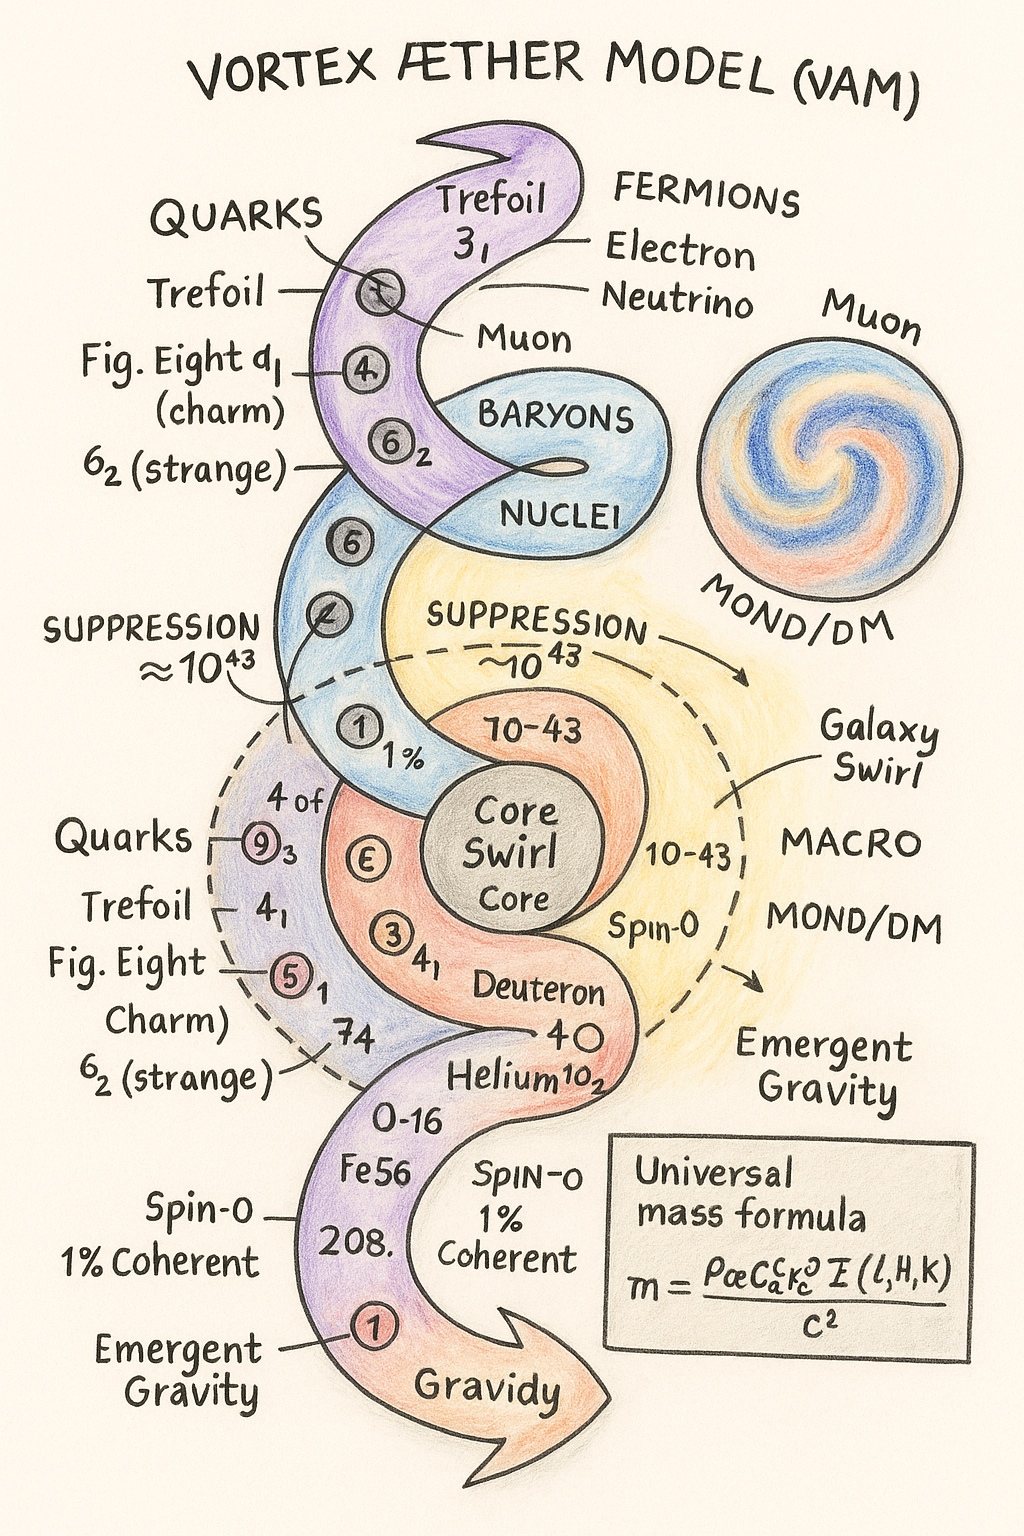
\includegraphics[width=0.85\textwidth]{images/ChatGPT Image Jul 15, 2025, 07_13_22 PM}
\caption{Your caption here.}
\end{figure}

\end{document}
